
\section{More Applications}
\subsection{Finding the Point of Intersection of Two Lines}

In this section, we will do application problems that involve the intersection of lines. Therefore, before we proceed any further, we will first learn how to find the intersection of two lines.

\begin{example}
Find the intersection of the line $y = 3x - 1$ and the line $y = -x + 7$.
\end{example}

\begin{solution}
We graph both lines on the same axes, as shown below, and read the solution $(2, 5)$.
\begin{center}
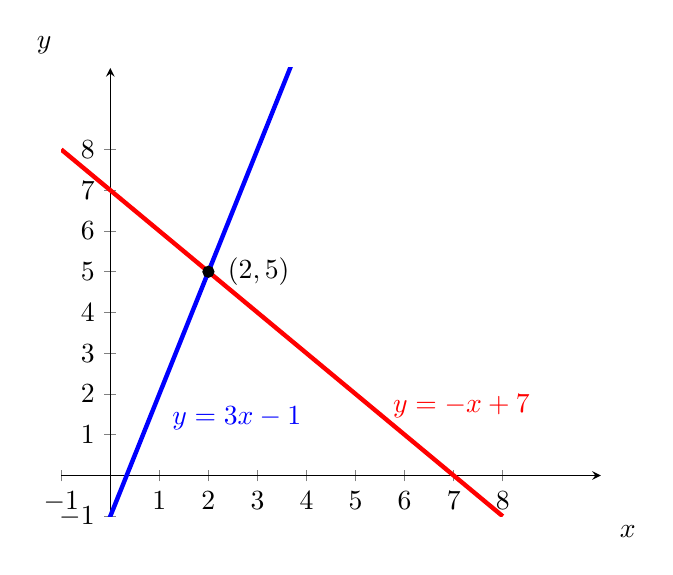
\begin{tikzpicture}[scale=1]
  \begin{axis}[
    axis lines=middle,
    xlabel={$x$},
    ylabel={$y$},
		xlabel style={at={(axis description cs:1.05,0)},anchor=north},
    ylabel style={at={(axis description cs:0,1.05)},anchor=east},
    xmin=-1, xmax=10,
    ymin=-1, ymax=10,
    xtick={-1,0,...,8},
    ytick={-1,0,...,8},
    samples=2,
  ]
  \addplot[blue, ultra thick, domain=-1:8]{3*x - 1} node[pos =.2, label={right:$y = 3x - 1$}] {};
  \addplot[red, ultra thick, domain=-1:8]{-x + 7} node[pos =.7, label={right:$y = -x + 7$}] {};
  \addplot[mark=*] coordinates {(2,5)} node[label={right:$(2, 5)$}] {};
  \end{axis}
\end{tikzpicture}
\end{center}

Finding an intersection of two lines graphically is not always easy or practical; therefore, we will now learn to solve these problems algebraically.

At the point where two lines intersect, the $x$ and $y$ values for both lines are the same. So in order to find the intersection, we either let the $x$-values or the $y$-values equal.

If we were to solve the above example algebraically, it will be easier to let the $y$-values equal. Since $y = 3x - 1$ for the first line, and $y = -x + 7$ for the second line, by letting the $y$-values equal, we get:

\begin{align*}
3x - 1 &= -x + 7 \\
4x &= 8 \\
x &= 2
\end{align*}

By substituting $x = 2$ in any of the two equations, we obtain $y = 5$. Hence, the solution is $(2, 5)$.
\end{solution}


\subsection{Solving Systems of Equations: The Elimination Method}

A common algebraic method used to solve systems of equations is called the elimination method. The objective is to eliminate one of the two variables by adding the left and right sides of the equations together. Once one variable is eliminated, we have an equation with only one variable that can be solved. Finally, by substituting the value of the variable that has been found in one of the original equations, we can get the value of the other variable.

\begin{example}
Find the intersection of the lines $2x + y = 7$ and $3x - y = 3$ by the elimination method.
\end{example}

\begin{solution}
We add the left and right sides of the two equations:

\begin{align*}
2x + y &= 7 \\
3x - y &= 3 \\
5x &= 10 \\
x &= 2
\end{align*}

Now we substitute $x = 2$ into any of the two equations and solve for $y$:

\begin{align*}
2(2) + y &= 7 \\
4 + y &= 7 \\
y &= 3
\end{align*}

Therefore, the solution is $(2, 3)$.
\end{solution}

\begin{example}
Solve the system of equations $x + 2y = 3$ and $2x + 3y = 4$ by the elimination method.
\end{example}

\begin{solution}
If we add the two equations directly, none of the variables are eliminated. However, the variable $x$ can be eliminated by multiplying the first equation by $-2$ and leaving the second equation unchanged:

\begin{align*}
-2x - 4y &= -6 \\
2x + 3y &= 4 \\
-y &= -2 \\
y &= 2
\end{align*}

Substituting $y = 2$ into $x + 2y = 3$, we get:

\begin{align*}
x + 2(2) &= 3 \\
x + 4 &= 3 \\
x &= -1
\end{align*}

Therefore, the solution is $(-1, 2)$.
\end{solution}

\begin{example}
Solve the system of equations $3x - 4y = 5$ and $4x - 5y = 6$.
\end{example}

\begin{solution}
This time, we multiply the first equation by $-4$ and the second by $3$ before adding (the choice of numbers is not unique):

\begin{align*}
-12x + 16y &= -20 \\
12x - 15y &= 18 \\
y &= -2
\end{align*}

By substituting $y = -2$ into any one of the equations, we get:

\begin{align*}
3x - 4(-2) &= 5 \\
3x + 8 &= 5 \\
3x &= -3 \\
x &= -1
\end{align*}

Hence, the solution is $(-1, -2)$.
\end{solution}

\subsection{Supply, Demand, and the Equilibrium Market Price}

In a free market economy, the supply curve for a commodity is the number of items of a product that can be made available at different prices, and the demand curve is the number of items the consumer will buy at different prices. As the price of a product increases, its demand decreases, and supply increases. On the other hand, as the price decreases, the demand increases, and supply decreases. The equilibrium price is reached when the demand equals the supply.

\begin{example}
The supply curve for a product is given by $y = 3.5x - 14$, and the demand curve for the same product is given by $y = -2.5x + 34$, where $x$ is the price and $y$ is the number of items produced. Find the following:
\begin{enumerate}
  \item How many items will be supplied at a price of \$10?
  \item How many items will be demanded at a price of \$10?
  \item Determine the equilibrium price.
  \item How many items will be produced at the equilibrium price?
\end{enumerate}
\end{example}

\begin{solution}
\begin{enumerate}
  \item To find the number of items supplied at a price of \$10, we substitute $x = 10$ into the supply equation $y = 3.5x - 14$. Therefore, $y = 3.5(10) - 14 = 21$ items will be supplied.
  
  \item To find the number of items demanded at a price of \$10, we substitute $x = 10$ into the demand equation $y = -2.5x + 34$. Therefore, $y = -2.5(10) + 34 = 9$ items will be demanded.
  
  \item To determine the equilibrium price, we set the supply equal to the demand:
  \[3.5x - 14 = -2.5x + 34\]
  Solving for $x$:
  \[6x = 48\]
  \[x = 8\]
  So, the equilibrium price is $x = 8$.
  
  \item To find how many items will be produced at the equilibrium price, we substitute $x = 8$ into either the supply or the demand equation. Using the supply equation, we get $y = 3.5(8) - 14 = 14$ items will be produced.
\end{enumerate}

The graph shows the intersection of the supply and demand functions and their point of intersection, $(8, 14)$.


\begin{center}
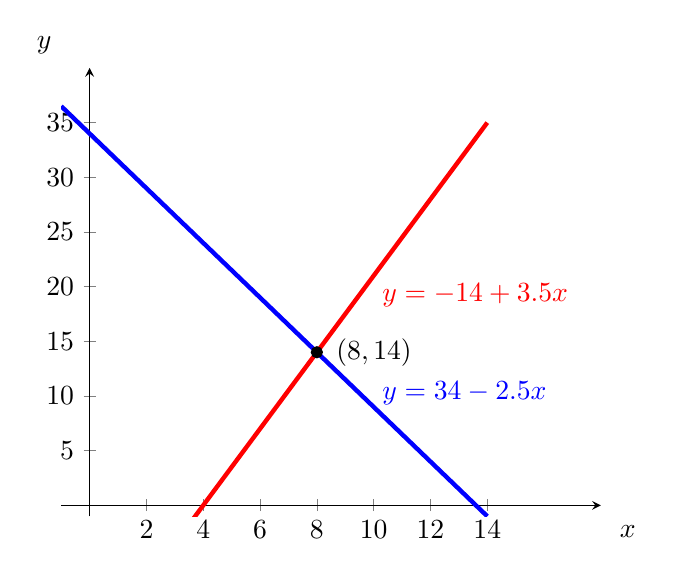
\begin{tikzpicture}[scale=1.0]
  \begin{axis}[
    axis lines=middle,
    xlabel={$x$},
    ylabel={$y$},
		xlabel style={at={(axis description cs:1.05,0)},anchor=north},
    ylabel style={at={(axis description cs:0,1.05)},anchor=east},
    xmin=-1, xmax=18,
    ymin=-1, ymax=40,
    xtick={0,2,...,14},
    ytick={0,5,...,35},
    samples=2,
  ]
  \addplot[blue, ultra thick, domain=-1:14]{34-2.5*x} node[pos =.7, label={right:$y = 34-2.5x$}] {};
  \addplot[red, ultra thick, domain=-1:14]{-14+3.5*x} node[pos =.7, label={right:$y = -14+3.5x$}] {};
  \addplot[mark=*] coordinates {(8,14)} node[label={right:$(8,14)$}] {};
  \end{axis}
\end{tikzpicture}
\end{center}

\end{solution}

\subsection{Break-Even Point}

In a business, profit is generated by selling products. If a company sells $x$ number of items at a price $P$, then the revenue $R$ is the price multiplied by the number of items sold: $R = P \cdot x$. The production costs $C$ are the sum of the variable costs and the fixed costs, often written as $C = mx + b$, where $x$ is the number of items manufactured.

\begin{itemize}
  \item The slope $m$ is called the marginal cost and represents the cost to produce one additional item or unit.
  \item The variable cost, $mx$, depends on how much is being produced.
  \item The fixed cost $b$ is constant and does not change regardless of production quantity.
\end{itemize}

Profit is equal to revenue minus cost: $Profit = R - C$. A company makes a profit if the revenue is greater than the cost, and there is a loss if the cost is greater than the revenue. The point on the graph where the revenue equals the cost is called the break-even point, and at this point, the profit is $0$.

\begin{example}
If the revenue function of a product is $R = 5x$ and the cost function is $C = 3x + 12$, find the following:
\begin{enumerate}
  \item If $4$ items are produced, what will the revenue be?
  \item What is the cost of producing $4$ items?
  \item How many items should be produced to break even?
  \item What will be the revenue and cost at the break-even point?
\end{enumerate}
\end{example}

\begin{solution}
\begin{enumerate}
  \item To find the revenue when $4$ items are produced, we substitute $x = 4$ in the revenue equation $R = 5x$, and the answer is $R = 20$.
  \item To find the cost of producing $4$ items, we substitute $x = 4$ in the cost equation $C = 3x + 12$, and the answer is $C = 24$.
  \item To determine the number of items required to break even, we set the revenue equal to the cost:
  \[5x = 3x + 12\]
  Solving for $x$:
  \[2x = 12\]
  \[x = 6\]
  So, $6$ items should be produced to break even.
  \item At the break-even point, when $x = 6$, we can substitute $x = 6$ in either the revenue or the cost equation to find that both revenue and cost are equal to $30$. Therefore, the revenue and cost at the break-even point are both $30$.
\end{enumerate}

The graph below shows the intersection of the revenue and cost functions and their point of intersection, $(6, 30)$.
\end{solution}

\begin{center}
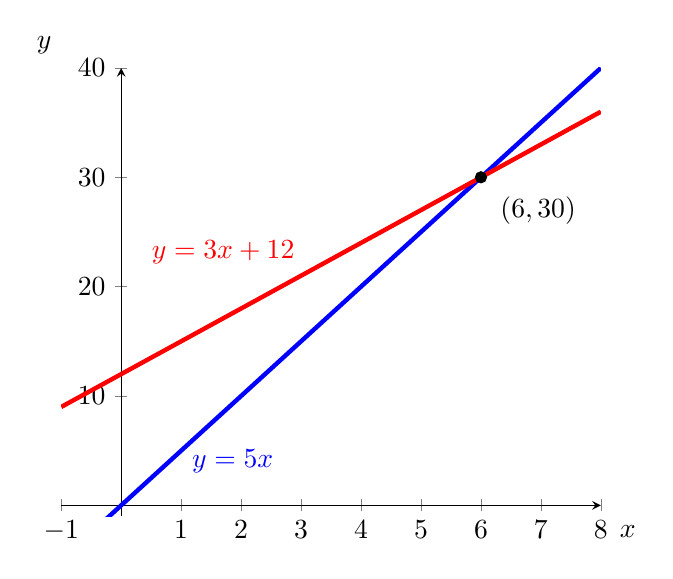
\begin{tikzpicture}[scale=1.0]
  \begin{axis}[
    axis lines=middle,
    xlabel={$x$},
    ylabel={$y$},
		xlabel style={at={(axis description cs:1.05,0)},anchor=north},
    ylabel style={at={(axis description cs:0,1.05)},anchor=east},
    xmin=-1, xmax=8,
    ymin=-1, ymax=40,
    xtick={-1,0,...,8},
    ytick={0,10,...,40},
    samples=2,
  ]
  \addplot[blue, ultra thick, domain=-1:8]{5*x} node[pos =.2, label={right:$y = 5x$}] {};
  \addplot[red, ultra thick, domain=-1:8]{3*x + 12} node[pos =.3, yshift=4mm, label={above:$y = 3x+12$}] {};
  \addplot[mark=*] coordinates {(6,30)} node[label={below right:$(6, 30)$}] {};
  \end{axis}
\end{tikzpicture}
\end{center}
